\begin{frame}
    \frametitle{Dijkstra}
    Let's go from $v_2$ to $v_3$
    \vfill
    \begin{columns}
    \column{0.5\textwidth}
    \centering
    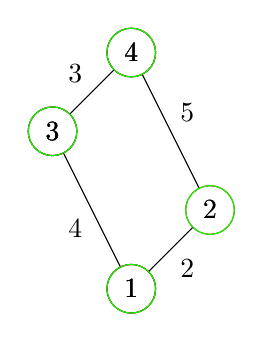
\begin{tikzpicture}[node distance={15mm}, main/.style = {draw, circle}]
        
        \onslide<1-2>{\node[main] (x3) at (0, 2) {$3$};}
        \onslide<3-4>{\node[main, draw=red] (x3) at (0, 2) {$3$};}
        \onslide<5->{\node[main, draw=green] (x3) at (0, 2) {$3$};}
        \onslide<1>{\node[main] (x4) at (1, 3) {$4$};}
        \onslide<2-3>{\node[main, draw=red] (x4) at (1, 3) {$4$};}
        \onslide<4->{\node[main, draw=green] (x4) at (1, 3) {$4$};}
        \onslide<1>{\node[main, draw=red] (x2) at (2, 1) {$2$};}
        \onslide<2->{\node[main, draw=green] (x2) at (2, 1) {$  2$};}
        \onslide<1>{\node[main] (x1) at (1, 0) {$1$};}
        \onslide<2>{\node[main, draw=red] (x1) at (1, 0) {$1$};}
        \onslide<3->{\node[main, draw=green] (x1) at (1, 0) {$1$};}
        
        \draw (x1) -- node[below right] {$2$}(x2);
        \draw (x1) -- node[below left] {$4$} (x3);
        \draw (x2) -- node[above right] {$5$} (x4);
        \draw (x3) -- node[above left] {$3$} (x4);

    \end{tikzpicture}
    \column{0.5\textwidth}
    \centering
    \begin{tabular}{c | c | c}
        \textbf{id} & \textbf{dist} & \textbf{settled}\\
        \hline 
        2 & 0  & \onslide<1>{false} \onslide<2->{true} \\ 
        \hline \pause
        1 & 2 & \onslide<2>{false} \onslide<3->{true}\\ 
        \hline
        4 &  5 & \onslide<2-3>{false} \onslide<4->{true} \\
        \hline \pause
        3 & 6 & \onslide<3-4>{false} \onslide<5->{true}\\ 
    \end{tabular}
\end{columns}
          
    

\end{frame}